\chapter{Design}\label{C:design}

The design process uses the goals of the experiment and the results of the initial evaluation to inform what and how various subsystems are designed.

From this there is a number of requirements to consider:

\begin{itemize}
    \item \textbf{Mechanical Stability}:
    \item \textbf{\dots}
    \item \textbf{System Expandability}:
\end{itemize}

\section{System Overview}

\begin{figure}[h]
    \begin{center}
        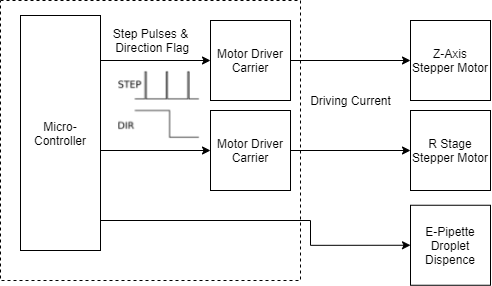
\includegraphics[width=0.5\textwidth]{img/ED_block_diag.png}
    \end{center}
\end{figure}

\section{Mechanical Design}

\begin{itemize}
    \item Discuss requirements for minimising settling time, vibrations, oscillations.overshoot of the pipette motion 
\end{itemize}

\subsection{Rotating Pipette Mount}

\begin{itemize}
    \item 3D printed pipette clamp
    \item Laser cut Tower mounted
    \item motor interface and stage fastening  
\end{itemize}

\subsection{Z micrometer Control}
\begin{itemize}
    \item Requirements: micrometer motion/extension as its turn
    \item Sliding motor shaft to knob required (2 passed)
    \item How it imposed restrictions on the system (freedom of motion)  
\end{itemize}

\section{Electronic Design}

\subsection{Motor Driving}

\subsubsection*{The Requirements}
To drive the selected stepper motors, discrete step/direction style micro stepping drivers were chosen. This allows for the design to be flexible with its electronics placed to accommodate the experimental needs. Allows for a fairly agnostic choice for controller to supply the control signals, and standardised pinouts allow for requirement flexibility and replacements.

\begin{table}[h]
    \centering
    \begin{tabular}{|l|l|l|l|l|}
        \hline
        \textbf{}     & \textbf{A4988} & \textbf{DRV8825} & \textbf{STPIN820} & \textbf{DRV8834} \\ \hline
        Step Res      & 1/16           & 1/32             & 1/256             & 1/32             \\ \hline
        Logic Level   & 3V3/5V         & 3V3/5V           & 3V3/5V            & 3V3/5V           \\ \hline
        Current Limit & 1A             & 1.5A             & 0.9A              & 1.5A             \\ \hline
        Drive Voltage & 8-35V          & 8.2-45V          & 7-48V             & 2.5-10.8         \\ \hline
    \end{tabular}
    \caption{Comparison of considered drivers}
\end{table}

Main consideration for device choice are: micro step resolution, driving current limit (passively cooled), and configuration pinout.

\subsubsection*{The Choice}
The DRV8825 was ultimately chosen.
\begin{itemize}
    \item High microstepping resolution, lower than the STPIN820 but cheap high resolution driver are prone to step skipping \cite{step_book}
    \item Highest driving current as torque requirements are unknown for this design the headroom is nice even if it isn't use, especially as it will run cooler at lower power draw.
    \item It ranked above the DRV8834 due to it configuration pins (to set microstepping mode) as it provide all 3 pins without the requirement to leave pins floating as a setting thus allowing for full software control.
\end{itemize}

\subsection{Pipette Triggering}

//TODO maybe move to implementation
\begin{itemize}
    \item Signal requirements that lead to a trigger environmental
    \item interfacing the controller with the board
\end{itemize}

\subsection{Environmental Monitoring}
\begin{itemize} 
    \item What will be measured?
    \item Power (battery?)
    \item Sleep the conserve
\end{itemize}
